% Poster Template with TikZ figures
% IMPORTANT: This template requires the sciposter class.
% For Overleaf: sciposter is available in TeX Live 2020+.
% Set compiler to pdflatex and main document to main.tex
% For local compilation: Install sciposter package or use Overleaf.
% Installation: tlmgr install sciposter (for TeX Live) or use package manager.
% !TeX program = pdflatex
% !TeX TXS-program:compile = txs:///pdflatex
\documentclass[36pt]{sciposter}
\usepackage{preposterTikz} % Style package with preamble
\geometry{paperwidth=90cm,paperheight=100cm,centering,
    textwidth=85cm,textheight=94cm,left=0cm,top=2cm}
\pgfplotsset{compat=1.18}
%********************************************************************
%********************************************************************
\begin{document}

\onehalfspacing

% Fill in the commands below with your information
% Format follows Springer LNCS style
\newcommand{\tituloposter}{Research Paper Title Research Paper Title Research Paper Title} % Main title (first line)
\newcommand{\titulogrande}{Research Paper Title} % Title continuation (second line, optional)
% NOTE: If you don't need a second line, leave the braces empty: \newcommand{\titulogrande}{}

% Author information - Springer LNCS format
% Format: First Author\inst{1}\orcidID{StudentID} \and Second Author\inst{1}\orcidID{StudentID}
% NOTE: For students, use Student ID instead of ORCID ID
\newcommand{\nome}{First Author\inst{1}\orcidID{20201234} \and Second Author\inst{1}\orcidID{20205678} \and Third Author\inst{1}\orcidID{20209012}}
\newcommand{\instituicao}{Faculty of Data Science and Artificial Intelligence,\\College of Technology, National Economics University\\\email{your.email@neu.edu.vn}}




% Simple plain header
\titulo{}{}{BoxCol} % Blue header background
% Note: Logo parameters are not used in the simple header format

\vspace{1cm} % Spacing

\section*{\tituloA{ABSTRACT}}

This section provides a brief summary of the research work, methodology, key findings, and conclusions. The abstract should be concise and informative, typically ranging from 150 to 250 words. It should give readers a clear understanding of the research objectives, approach, and main contributions without requiring them to read the entire poster.


% Two-column layout
\begin{multicols}{2}

% Paragraph indentation
\setlength{\parindent}{3em}

\section*{\tituloA{OBJECTIVES}}

\noindent
The objectives section should clearly state the research goals and what the study aims to achieve. This may include:

\begin{itemize}
\item Primary research objectives
\item Specific research questions to be addressed
\item Expected outcomes or contributions
\item Scope and limitations of the study
\end{itemize}



\section*{\tituloA{METHODOLOGY}}

This section describes the research methodology, experimental design, data collection procedures, and analytical approaches used in the study. It should provide sufficient detail for readers to understand how the research was conducted.

% Springer LNCS style figure format - Proposed framework visualization
Figure~\ref{fig:method} illustrates the overall architecture and workflow of the proposed method.

\begin{figure}
\centering
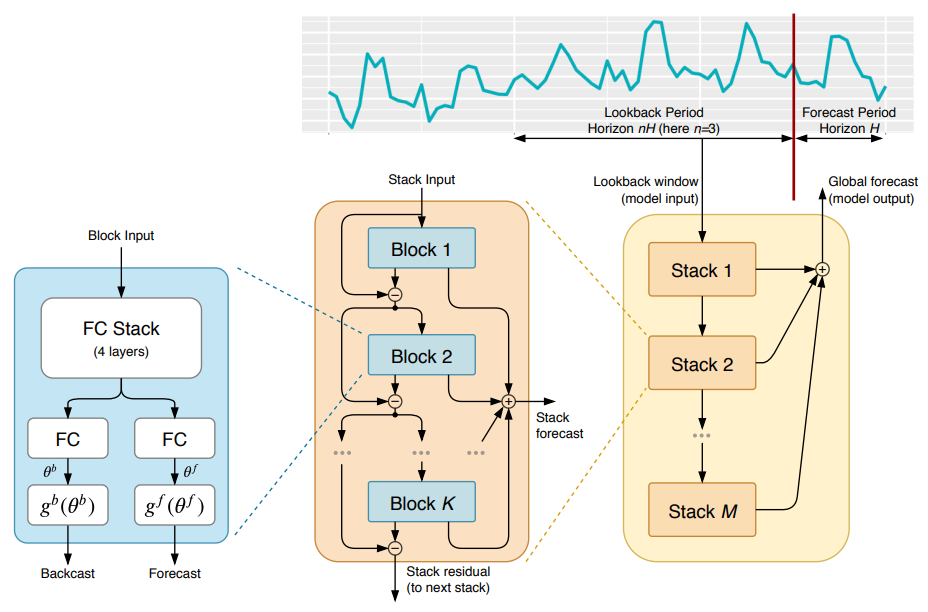
\includegraphics[width=\textwidth]{Figures/sample_method_fig.png}
\caption{Overview of the proposed method architecture and workflow.} \label{fig:method}
\end{figure}

The methodology may include theoretical frameworks, algorithms, experimental setups, or analytical techniques. Additional methodological details, data sources, software tools, and implementation specifics should be described here.



\section*{\tituloA{RESULTS}}

This section presents the main findings of the research. Results should be presented clearly using tables and descriptive text. Key findings should be highlighted and discussed in the context of the research objectives.

% Springer LNCS style table format
Table~\ref{tab1} presents a comparison of different methods.

\begin{table}
\caption{Comparison of different approaches.}\label{tab1}
\centering
\begin{tabular}{|l|l|l|}
\hline
Method & Metric 1 & Metric 2\\
\hline
Baseline & 0.XX & 0.XX\\
Method A & 0.XX & 0.XX\\
Proposed & 0.XX & 0.XX\\
\hline
\end{tabular}
\end{table}

Additional results, statistical analyses, and comparative evaluations should be presented here to support the main findings.



\section*{\tituloA{CONCLUSIONS}}

This section summarizes the main conclusions drawn from the research. It should:

\begin{itemize}
\item Restate the key findings in relation to the research objectives
\item Discuss the significance and implications of the results
\item Address any limitations encountered during the study
\item Suggest potential future research directions
\end{itemize}

The conclusions should provide a clear and concise summary that ties together all aspects of the research presented in the poster.


\section*{\tituloA{REFERENCES}}
\begin{enumerate}
	\item[[1]] Author, A. B., \& Author, C. D. (Year). Title of the article. \textit{Journal Name}, \textbf{Volume}(Issue), pages--pages. DOI: 10.xxxx/xxxxx
	
	\item[[2]] Author, E. F. (Year). \textit{Book Title} (Edition). Publisher, Location.
	
	\item[[3]] Author, G. H., Author, I. J., \& Author, K. L. (Year). Conference paper title. In \textit{Conference Name} (pp. pages--pages). Publisher.
	
	\item[[4]] Author, M. N. (Year). Website or online resource. Retrieved from \texttt{http://example.com}
\end{enumerate}


\end{multicols}

\end{document}